\section{Buildroot}
% ----
\subsection{Répertoires}
\begin{figure}[H]
    \centering
    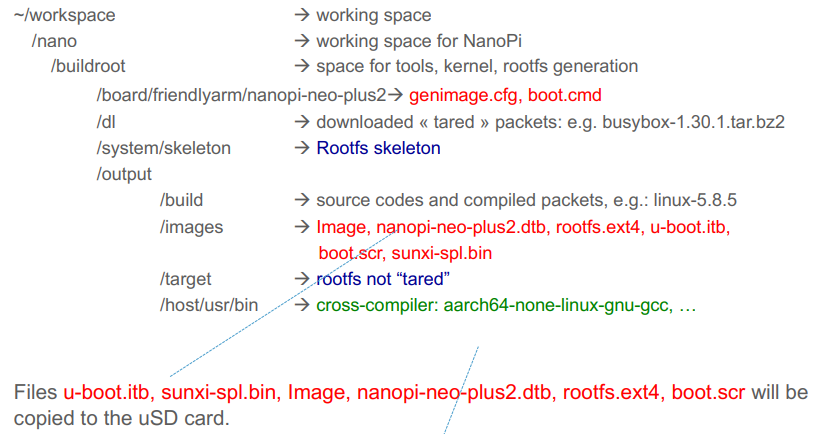
\includegraphics[width=\linewidth]{buildroot_dir.png}
\end{figure}

\begin{itemize}
\item \texttt{board/}: contient les fichiers de configuration pour les différentes cartes matérielles prises en charge par Buildroot.
\item \texttt{package/}: contient les fichiers de configuration pour les différents paquets logiciels qui peuvent être inclus dans l'image de système.
\item \texttt{toolchain/}: contient les fichiers de configuration pour les différents outils de compilation (comme les compilateurs et les bibliothèques) qui peuvent être utilisés pour construire l'image de système.
\item \texttt{output/}: contient les fichiers générés lors de la construction de l'image de système, tels que les images d'amorçage, les fichiers système de fichiers, etc.
\item \texttt{configs/}: contient les fichiers de configuration de base pour les différents systèmes d'exploitation pris en charge par Buildroot.
\item \texttt{target/}: contient les fichiers générés pour la cible (comme les bibliothèques, les exécutables, les fichiers de configuration, etc.)
\item \texttt{support/}: contient des scripts et des fichiers de configuration supplémentaires utilisés par Buildroot.
\end{itemize}

\verb+make+ compile les fichiers manquant au dossier \verb+output+ (compiler que un paquet avec \verb+make <package>-rebuild+).
%
\subsection{Configuration $\rightarrow$ Compilation}
\begin{itemize}
    \item paramétré avec \verb+make menuconfig+

    \item Sauvée dans \begin{itemize}
        \item \verb+/buildroot/.config+ : full default config file
        \item \verb+/buildroot/xxx_defconfig+ : stores only the values for options for which the non-default value is chosen
        \end{itemize}
\end{itemize}

\subsubsection{Patch}
\begin{itemize}
    \item \verb+git checkout -b [new feature branch]+
    \item \verb+git commit -am "Description of modif."+
    \item \verb+git format-patch [main branch name]+
\end{itemize}
Une option dans \verb+make menuconfig+ permet de définir un dossier dans lequel se trouvent les patchs à appliquer (Build options $\rightarrow$ global patch directories $\rightarrow$ p.ex. \verb+/board/friendlyarm/nanopi-.../patches+)
% ----
\subsection{Carte SD}
\begin{figure}[H]
    \centering
    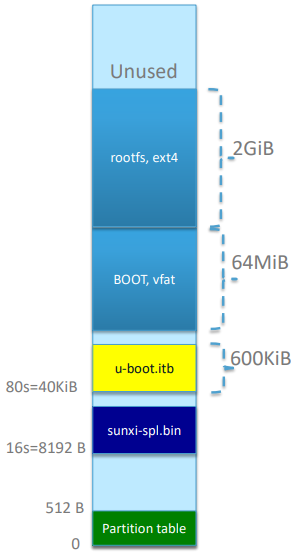
\includegraphics[height=\columnwidth, angle=90]{SD_card.png}
\end{figure}
\begin{itemize}
    \item \verb+rootfs+ : \verb+/bin+, \verb+/sbin+, \verb+/root+, etc.
    \item \verb+BOOT+ : \verb+Image+, \verb+nanopi-neo-plus2.dtb+, \verb+boot.scr+.
\end{itemize}
%\begin{figure}[H]
%    \centering
%    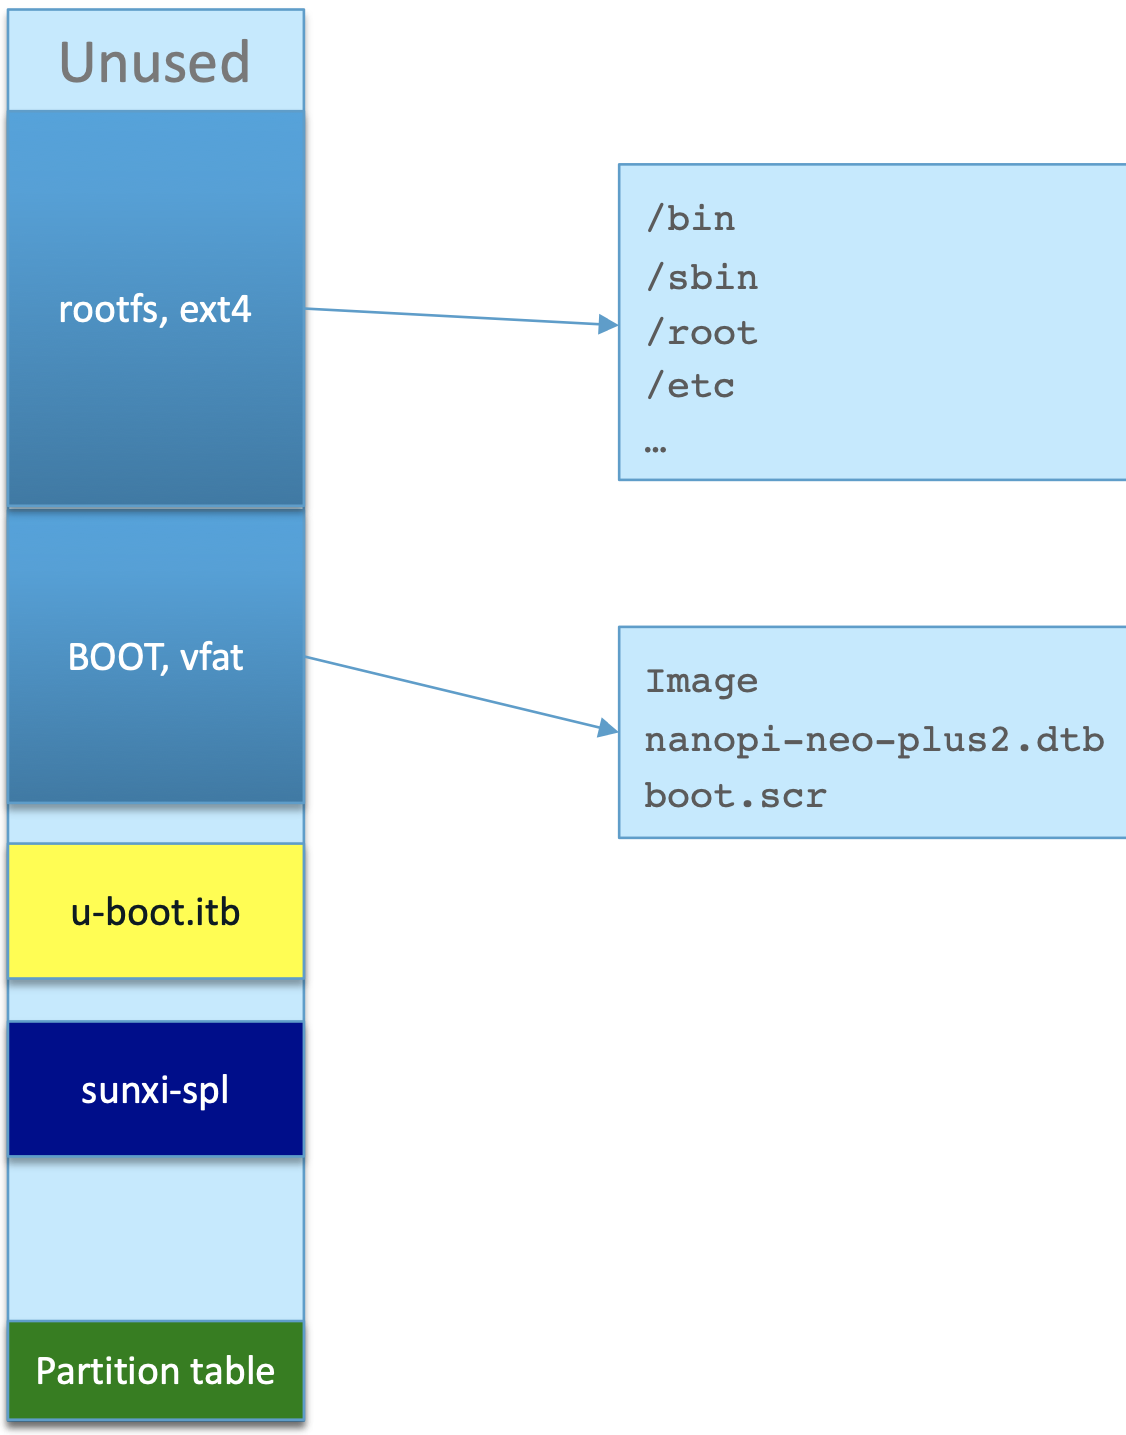
\includegraphics[height=\columnwidth, angle=90]{boot_rootfs_content.png}
%\end{figure}
\begin{center}
\verb!genimage.cfg!$\rightarrow$\verb!genimage!$\rightarrow$\verb!sdcard.img!$\rightarrow$\verb!dd!$\rightarrow$ carte SD
\end{center}
Les fichiers pour l'initialisation sont\\
\begin{table}[H]
\begin{tabular}{lp{4cm}}
\verb!rootfs.ext! & Root file system\\
\verb!Image! & Noyau Linux\\
\verb!nanopo-neo-plus2.dtb! & Flattened device tree\\
\verb!boot.scr! & Commandes boot compilées utilisées par u-boot\\
\verb!boot.vfat! & Partition boot\\
\verb!u-boot.itb! & Boot loader\\
\verb!sunxi-spl.bin! & Secondary Program Loader
\end{tabular}
\end{table}
\verb!boot.vfat! contient \verb!Image!, \verb!nanopi-neo-plus2.dtb! et \verb!boot.scr!. \verb!boot.vfat! (ou \verb!boot.ext4!) permet de créer \verb!BOOT! sur la carte SD
\subsubsection{rootfs}
Fichier dans un certain format (p.ex. \verb+.ext4+), organisé comme une partition.
Contient \verb!/bin!, \verb!/sbin!, \verb!/root!, \verb!/etc!, etc...
\subsubsection{rootfs\_overlay}
Permet de personnaliser un système de fichiers en utilisant des répertoires supplémentaires pour écraser ou ajouter des fichiers au système de fichiers de base généré par Buildroot.
\subsubsection{boot.scr}
Le fichier \verb!boot.scr! est utilisé par u-boot pour charger le kernel Linux. Il est créé avec la commande \verb!mkimage!
\subsubsection{boot.cmd}
\verb!boot.cmd! contient des informations de démarrage, notamment les emplacements des différents l'emplacement de \verb!nanopi-neo-plus2.dtb!, du kernel et (si présent) de l'initramfs

\subsection{Installer un package}
Package se trouvent dans \verb+/buildroot/packages+
Contient :
\begin{itemize}
    \item \verb+Config.in+ file, written in kconfig language, describing the configuration options for the package.
    \item \verb+foo.mk+ makefile, describing where to fetch the source, how to build and install it, etc.
    \item \verb+Sxx_foo+ it is the start script for the foo package.
\end{itemize}